\documentclass[xetex,mathserif,serif]{beamer}
\usepackage{polyglossia}
\setdefaultlanguage[babelshorthands=true]{russian}
\usepackage{minted}
\usepackage{tabu}

\useoutertheme{infolines}

\usepackage{fontspec}
\setmainfont{FreeSans}
\newfontfamily{\russianfonttt}{FreeSans}

\definecolor{links}{HTML}{2A1B81}
\hypersetup{colorlinks,linkcolor=,urlcolor=links}

\setbeamertemplate{blocks}[rounded][shadow=false]
\setbeamercolor*{block title alerted}{fg=red!50!black,bg=red!20}
\setbeamercolor*{block body alerted}{fg=black,bg=red!10}

\tabulinesep=0.8mm

\title{Низкоуровневые потоки, события}
\author{Юрий Литвинов}
\date{17.04.2018г}

\begin{document}

	\frame{\titlepage}

	\section{Доклады}

	\begin{frame}
		\frametitle{Доклады}
		\framesubtitle{Минус одна домашка}
		\begin{itemize}
			\item Дополнительные возможности F\# (единицы измерения, lazy, active patterns)
			\item F\# и анализ данных
			\item WebSharper (обзор и небольшая демонстрация)
			\item Type Providers, F\# Data
			\item FAKE, Scaffold
		\end{itemize}
	\end{frame}

	\section{Потоки}

	\begin{frame}
		\frametitle{Потенциальные проблемы с потоками}
		\begin{itemize}
			\item Гонки (Race condition)
				\begin{center}
					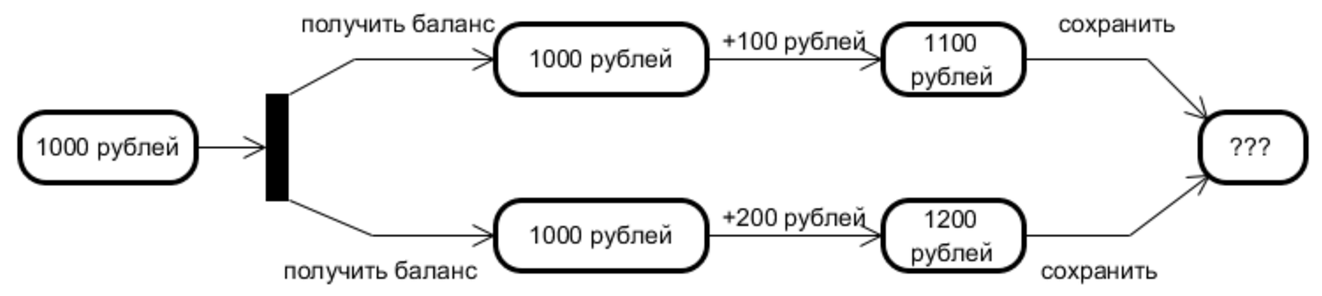
\includegraphics[width=0.8\textwidth]{raceCondition.png}
				\end{center}
				\vspace{1cm}
			\item Тупики (Deadlock)
				\begin{center}
					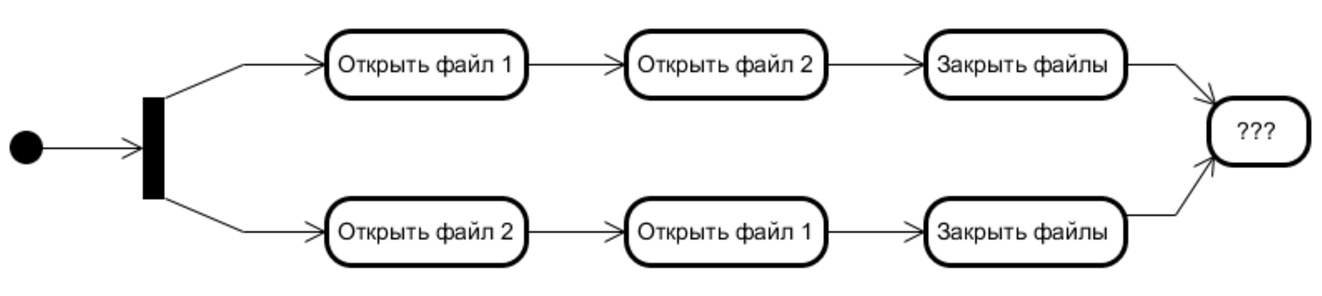
\includegraphics[width=0.8\textwidth]{deadlock.png}
				\end{center}
		\end{itemize}
	\end{frame}

	\begin{frame}[fragile]
		\frametitle{Пример гонки}
		\begin{minted}{fsharp}
open System.Threading

type MutablePair<'a,'b>(x:'a, y:'b) =
    let mutable currentX = x
    let mutable currentY = y
    member p.Value = (currentX, currentY)
    member p.Update(x, y) =
        currentX <- x
        currentY <- y

let p = MutablePair (0, 0)
Async.Start (async { while true do p.Update(10, 10) })
Async.Start (async { while true do p.Update(20, 20) })

Async.RunSynchronously (async { while true do printfn "%A" p.Value })
		\end{minted}
	\end{frame}

	\begin{frame}
		\frametitle{Примитивы синхронизации}
		\begin{itemize}
			\item Лучше необходимости синхронизации вообще избегать
			\item Бывают:
			\begin{itemize}
				\item User-mode --- атомарные операции, реализующиеся на процессоре и не требующие участия планировщика
				\item Kernel-mode --- примитивы, управляющие тем, как поток обрабатывается планировщиком
				\begin{itemize}
					\item Более тяжеловесные и медленные (до 1000 раз по сравнению с ``без синхронизации вообще'')
					\item Позволяют синхронизировать даже разные процессы
				\end{itemize}
			\end{itemize}
		\end{itemize}
	\end{frame}

	\begin{frame}[fragile]
		\frametitle{Пример примитива синхронизации: монитор}
		\begin{minted}{fsharp}
let lock (lockobj : obj) f =
    Monitor.Enter lockobj
    try
        f()
    finally
        Monitor.Exit lockobj

Async.Start (async { 
    while true do lock p (fun () -> p.Update(10, 10)) })

Async.Start (async { 
    while true do lock p (fun () -> p.Update(20, 20)) })
		\end{minted}
	\end{frame}

	\begin{frame}
		\frametitle{Примитивы синхронизации}
		\framesubtitle{Пространство имён System.Threading}
		\begin{footnotesize}
			\begin{tabu} {| X[0.3 l p] | X[1 l p] |}
				\tabucline-
				Примитив          & Описание           \\
				\tabucline-
				\everyrow{\tabucline-}
				AutoResetEvent    & Точка синхронизации. WaitOne блокирует поток, пока кто-нибудь другой не вызовет Set.  \\
				ManualResetEvent  & То же, что AutoResetEvent, но сбрасывается вручную, вызовом Reset                     \\
				Monitor           & Ограничивает доступ к критической секции                                              \\
				Mutex             & Ограничивает доступ к критической секции, работает между процессами                   \\
				Semaphore         & Позволяет находиться в критической секции не более N потоков                          \\
				Interlocked       & Атомарные арифметические операции                                                     \\
			\end{tabu}
		\end{footnotesize}
	\end{frame}

	\begin{frame}
		\frametitle{Управление планировщиком}
		\begin{small}
			\begin{itemize}
				\item \mintinline{fsharp}|Thread.Sleep(0)| --- ничего не делает, если остальные готовые потоки меньше приоритетом
				\item \mintinline{fsharp}|Thread.Sleep(1)| --- отдаёт управление потоку, даже если его приоритет меньше
				\item \mintinline{fsharp}|Thread.Yield()| --- нечто среднее (не вызовет переключения потоков, если желающих нет, в отличие от \mintinline{fsharp}|Thread.Sleep(1)|, но отдаст ядро потоку с меньшим приоритетом)
				\item \mintinline{fsharp}|Thread.SpinWait()| --- подождать в цикле, не переключая контексты
				\item Очередной способ прострелить себе ногу --- инверсия приоритетов
				\begin{itemize}
					\item Поток с низким приоритетом захватил ресурс, нужный потоку с высоким приоритетом
					\item Поток с высоким приоритетом крутится в ожидании, никогда не отдавая управление потоку, который мог бы отдать ресурс (livelock)
				\end{itemize}
			\end{itemize}
		\end{small}
	\end{frame}

	\begin{frame}[fragile]
		\frametitle{BackgroundWorker}
		\framesubtitle{Более высокоуровневый способ работы с потоками}
		\begin{minted}{fsharp}
let worker = new BackgroundWorker()
let numIterations = 1000

worker.DoWork.Add(fun args ->
    let rec computeFibonacci resPrevPrev resPrev i =
        let res = resPrevPrev + resPrev
        
        if i = numIterations then
            args.Result <- box res
        else
            computeFibonacci resPrev res (i + 1)

    computeFibonacci 1 1 2)
		\end{minted}
\end{frame}

	\begin{frame}[fragile]
		\frametitle{BackgroundWorker, как запустить}
		\begin{minted}{fsharp}
worker.RunWorkerCompleted.Add(fun args ->
    MessageBox.Show (sprintf "Result = %A" 
        args.Result) |> ignore)

worker.RunWorkerAsync()
		\end{minted}
	\end{frame}

	\section{События}

	\begin{frame}[fragile]
		\frametitle{События}
		\begin{alertblock}{F\# Interactive}
			\begin{minted}{fsharp}
> open System.Windows.Forms;;
> let form = new Form(Text="Click Form",  
                      Visible=true,TopMost=true);;
val form : Form

> form.Click.Add(fun evArgs -> printfn "Clicked!");;
val it : unit = ()

> form.MouseMove.Add(fun args -> printfn "Mouse, 
                     (X,Y) = (%A,%A)" args.X args.Y);;
val it : unit = ()
			\end{minted}
		\end{alertblock}
\end{frame}

	\begin{frame}[fragile]
		\frametitle{Microsoft.FSharp.Control.Event}
		\begin{minted}{fsharp}
Form.MouseMove
    |> Event.filter (fun args -> args.X > 100)
    |> Event.add (fun args -> printfn "Mouse, 
                  (X,Y) = (%A,%A)" args.X args.Y)
		\end{minted}
	\end{frame}

	\begin{frame}
		\frametitle{Что ещё с ними можно делать}
		\begin{footnotesize}
			\begin{tabu} {| X[0.3 l p] | X[1 l p] |}
				\tabucline-
				Примитив  & Описание           \\
				\tabucline-
				\everyrow{\tabucline-}
				add       & ('T $\to$ unit) $\to$ IEvent<'Del,'T> $\to$ unit                                 \\
				filter    & ('T $\to$ bool) $\to$ IEvent<'Del,'T> $\to$ IEvent<'T>                           \\
				choose    & ('T $\to$ 'U option) $\to$ IEvent<'Del,'T> $\to$ IEvent<'U>                      \\
				map       & ('T $\to$ 'U) $\to$ IEvent<'Del, 'T> $\to$ IEvent<'U>                            \\
				merge     & IEvent<'Del1,'T> $\to$ IEvent<'Del2,'T> $\to$ IEvent<'T>                         \\
				pairwise  & IEvent<'Del,'T> $\to$ IEvent<'T * 'T>                                            \\
				partition & ('T $\to$ bool) $\to$ IEvent<'Del,'T> $\to$ IEvent<'T> * IEvent<'T>              \\
				scan      & ('U $\to$ 'T $\to$ 'U) $\to$ 'U $\to$ IEvent<'Del,'T> $\to$ IEvent<'U>           \\
				split     & ('T $\to$ Choice<'U1,'U2>) $\to$ IEvent<'Del,'T> $\to$ IEvent<'U1> * IEvent<'U2> \\
			\end{tabu}
		\end{footnotesize}
	\end{frame}

	\begin{frame}[fragile]
		\frametitle{Как описывать свои события}
		\begin{minted}{fsharp}
open System
open System.Windows.Forms

type RandomTicker(approxInterval) =
    let timer = new Timer()
    let rnd = new System.Random 99
    let tickEvent = new Event<_>()

    let chooseInterval() :int =
        approxInterval + approxInterval / 4
               - rnd.Next(approxInterval / 2)

    do timer.Interval <- chooseInterval()
		\end{minted}
\end{frame}

	\begin{frame}[fragile]
		\frametitle{Как описывать свои события (2)}
		\begin{minted}{fsharp}
do timer.Tick.Add(fun args ->
    let interval = chooseInterval()
    tickEvent.Trigger(interval)
    timer.Interval <- interval)

member x.RandomTick = tickEvent.Publish
member x.Start() = timer.Start()
member x.Stop() = timer.Stop()

interface IDisposable with
    member x.Dispose() = timer.Dispose()
		\end{minted}
	\end{frame}

	\begin{frame}[fragile]
		\frametitle{Пример использования}
		\begin{alertblock}{F\# Interactive}
			\begin{minted}{fsharp}
> let rt = new RandomTicker(1000);;
val rt : RandomTicker
> rt.RandomTick.Add(fun nextInterval -> printfn "Tick, 
        next = %A" nextInterval);;
val it : unit = ()

> rt.Start();;
Tick, next = 1072
Tick, next = 927
Tick, next = 765
...
val it : unit = ()
> rt.Stop();;
val it : unit = ()
			\end{minted}
		\end{alertblock}
	\end{frame}

	\begin{frame}[fragile]
		\frametitle{Свой worker, с событиями}
		\begin{minted}{fsharp}
open System.ComponentModel
open System.Windows.Forms

type IterativeBackgroundWorker<'a>(oneStep:('a -> 'a),
        initialState:'a,
        numIterations:int) =
    let worker =
        new BackgroundWorker(WorkerReportsProgress = true,
            WorkerSupportsCancellation = true)

    let completed = new Event<_>()
    let error = new Event<_>()
    let cancelled = new Event<_>()
    let progress = new Event<_>()
		\end{minted}
\end{frame}

	\begin{frame}[fragile]
		\frametitle{Свой worker (2)}
		\begin{minted}{fsharp}
do worker.DoWork.Add(fun args ->
let rec iterate state i =
    if worker.CancellationPending then
        args.Cancel <- true
    elif i < numIterations then
        let state' = oneStep state
        let percent = int ((float (i + 1) 
            / float numIterations) * 100.0)
        do worker.ReportProgress(percent, box state);
        iterate state' (i + 1)
    else
        args.Result <- box state

iterate initialState 0)
		\end{minted}
	\end{frame}

	\begin{frame}[fragile]
		\frametitle{Свой worker (3)}
		\begin{minted}{fsharp}
do worker.RunWorkerCompleted.Add(fun args ->
    if args.Cancelled then cancelled.Trigger ()
    elif args.Error <> null then error.Trigger args.Error
    else completed.Trigger (args.Result :?> 'a))

do worker.ProgressChanged.Add(fun args ->
    progress.Trigger (args.ProgressPercentage, (args.UserState :?> 'a)))

member x.WorkerCompleted = completed.Publish
member x.WorkerCancelled = cancelled.Publish
member x.WorkerError = error.Publish
member x.ProgressChanged = progress.Publish

member x.RunWorkerAsync() = worker.RunWorkerAsync()
member x.CancelAsync() = worker.CancelAsync()
		\end{minted}
	\end{frame}

	\begin{frame}[fragile]
		\frametitle{Тип того, что получилось}
		\begin{minted}{fsharp}
type IterativeBackgroundWorker<'a> =
  class
    new : oneStep:('a -> 'a) 
            * initialState:'a 
            * numIterations:int 
            -> IterativeBackgroundWorker<'a>
    member CancelAsync : unit -> unit
    member RunWorkerAsync : unit -> unit
    member ProgressChanged : Event<int * 'a>
    member WorkerCancelled : Event<unit>
    member WorkerCompleted : Event<'a>
    member WorkerError : Event<exn>
  end
		\end{minted}
	\end{frame}

	\begin{frame}[fragile]
		\frametitle{Пример использования}
		\begin{minted}{fsharp}
let fibOneStep (fibPrevPrev:bigint,fibPrev) = 
                  (fibPrev, fibPrevPrev + fibPrev)

let worker = new IterativeBackgroundWorker<_>(fibOneStep,
             (1I, 1I), 100)

worker.WorkerCompleted.Add(fun result ->
  MessageBox.Show(sprintf "Result = %A" result) |> ignore)

worker.ProgressChanged.Add(fun (percentage, state) ->
  printfn "%d%% complete, state = %A" percentage state)

worker.RunWorkerAsync()
		\end{minted}
	\end{frame}

	\begin{frame}[fragile]
		\frametitle{Своё новое событие}
		\begin{footnotesize}
			\begin{minted}{fsharp}
open System
open System.Threading

type IterativeBackgroundWorker<'a>(...) =
    let worker = ...

    let syncContext = SynchronizationContext.Current
    do if syncContext = null then failwith 
        "no synchronization context found"
    
    let started = new Event<_>()

    do worker.DoWork.Add(fun args ->
        syncContext.Post(SendOrPostCallback(fun _ -> 
            started.Trigger(DateTime.Now)),
            state=  null))
    ...
    member x.Started = started.Publish
			\end{minted}
		\end{footnotesize}
	\end{frame}

	\section{Lock-free}

	\begin{frame}
		\frametitle{Атомарные операции}
		\begin{itemize}
			\item Нет синхронизации --- нет deadlock-ов!
			\item Чтения и записи следующих типов всегда атомарны: Boolean, Char, (S)Byte, (U)Int16, (U)Int32, (U)IntPtr, Single, ссылочные типы
			\item Volatile
			\begin{itemize}
				\item Volatile.Write
				\item Volatile.Read
				\item Связано с понятием Memory Fence, требует синхронизации ядер
				\item Есть атрибут VolatileField
				\item Volatile.Write должен быть последней операцией записи, Volatile.Read --- первой операцией чтения
			\end{itemize}
		\end{itemize}
	\end{frame}

	\begin{frame}[fragile]
		\frametitle{Пример}
		\begin{minted}{fsharp}
let mutable flag = 0
let mutable value = 0

let thread1 () = 
    value <- 5
    Volatile.Write(ref flag, 1)

let thread2 () =
    if Volatile.Read(ref flag) = 1 
    then
        printfn "%d" value;
		\end{minted}
	\end{frame}

	\begin{frame}
		\frametitle{Синхронизация ядер, метафора}
		\framesubtitle{Relaxed ordering}
		\begin{columns}
			\begin{column}{0.6\textwidth}
				\begin{itemize}
					\item Каждую атомарную переменную можно понимать как список значений
					\item Каждый поток может спросить текущее значение, переменная вернёт ЛЮБОЕ значение из списка (текущее или одно из предыдущих)
				\end{itemize}
			\end{column}
			\begin{column}{0.4\textwidth}
				\begin{center}
					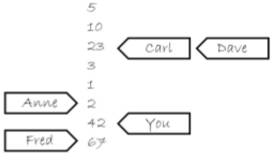
\includegraphics[width=0.7\textwidth]{relaxedOrdering.png}
				\end{center}
			\end{column}
		\end{columns}
		\begin{itemize}
			\item Переменная ``запомнит'', какое значение она вернула этому потоку
			\item Когда поток спросит значение в следующий раз, она вернёт ЛЮБОЕ значение между текущим и последним, которое она вернула ЭТОМУ потоку
		\end{itemize}
	\end{frame}

	\begin{frame}
		\frametitle{Interlocked}
		\begin{itemize}
			\item Одновременные чтение и запись в одной ``транзакции''
			\begin{itemize}
				\item \mintinline{fsharp}|Increment : location:int byref -> int|
				\item \mintinline{fsharp}|Decrement : location:int byref -> int|
				\item \mintinline{fsharp}|Add : location1:int byref * value:int -> int|
				\item \mintinline{fsharp}|Exchange : location1:int byref * value:int -> int|
				\item \mintinline{fsharp}|CompareExchange|
						\mintinline{fsharp}|        : location1:int byref * value:int * comparand:int -> int|
			\end{itemize}
		\end{itemize}
	\end{frame}

	\begin{frame}[fragile]
		\frametitle{Interlocked lock-free-максимум}
		\begin{footnotesize}
			\begin{minted}{fsharp}
let maximum target value =
    let mutable currentVal = target
    let mutable startVal = 0
    let mutable desiredVal = 0
    let mutable isDone = false
    while not isDone do
        startVal <- currentVal
        desiredVal <- max startVal value
        // Тут другой поток мог уже испортить target, так что если она изменилась,
        // надо начать всё сначала.
        currentVal <- Interlocked.CompareExchange(ref target, desiredVal, startVal)
        if startVal = currentVal then
            isDone <- true
    desiredVal
			\end{minted}
		\end{footnotesize}
	\end{frame}

\end{document}
